
%\documentclass[]{algotel}
%\usepackage[utf8]{inputenc}
\documentclass[10pt, conference, letterpaper]{IEEEtran}
%
\usepackage[utf8]{inputenc}
\usepackage[english]{babel}
\usepackage{caption}
\usepackage{authblk}
\usepackage{graphicx}

\usepackage{xspace}
\usepackage{graphics}
\usepackage{mathtools, bm}

\usepackage{amssymb, bm}
\usepackage{complexity}
\usepackage{amsmath,amsthm}

\usepackage{color}
\usepackage{amsmath}
%\usepackage[colorlinks=true,breaklinks=true,linkcolor=blue]{hyperref}
\captionsetup{justification=centering,margin=0.5cm}


\newcommand\pall{\textsc{pall}\xspace}
\newcommand{\todo}[1]{{\color{red} TODO: {#1}}}
\newtheorem{prop}{Proposition}

\newtheorem{theorem}{Theorem}
\newtheorem{corollary}{Corollary}[theorem]

\renewcommand{\thefootnote}{\*}

\graphicspath{{img/}}
\title{Deterministic latency for Cloud RAN over an optical ring}


\author[1]{Dominique Barth}
\author[1,2]{Ma\"el Guiraud}
\author[1]{Yann Strozecki}
\affil[1]{David Laboratory, UVSQ}
\affil[2]{Nokia Bell Labs France}

\begin{document}

\maketitle


\begin{abstract}
The N-GREEN project has for goal to design a low cost optical ring technology with good performances (throughput, latency$\dots$) without using expensive end to end connections. We study the compatibility of such a technology with the development of the Cloud RAN, a latency critical application which is a major aspect of 5G deployment. We show that deterministically managing Cloud RAN traffic minimizes its latency while also improving the latency of the other traffics.

\end{abstract}


\section{Introduction}

\footnote{This work was developed around the ANR N-GREEN project.}  Telecommunication network providers have to design inexpensive networks supporting an increasing amount of data and online applications. Much of these applications require QoS guarantees, like a minimal throughput and/or  a maximal latency. The N-GREEN project aims to design a high performing packet-switching optical ring while ensuring a minimal cost for providers. The current solutions with good QoS~\cite{pizzinat2015things,tayq2017real}, establish end to end direct connections (E2DE) between the nodes, which is extremely expensive. The N-GREEN optical ring is designed to ensure good performance: the hardware it requires scales linearly with the number of nodes while E2DE scales quadratically making it impractical for more than a few nodes.


In this article, we focus on a Cloud RAN application (C-RAN) on the N-GREEN optical ring described in ~ \cite{ngreenarchitecture, uscumlicscalable}. C-RAN is one of the main areas of development of 5G; it consists in centralizing or partially centralizing the computation units or BaseBand Units (BBU) of the Remote Radio Heads (RRH) in a datacenter. This application therefore requires periodic uplink and downlink communications of data frames between  all the  RRH and their corresponding BBU; the period and the latency must be fixed in time, if possible  minimum, in order to respect the time constraints of the application. In particular, the end-to-end latency must be less than or equal to $ 1 $ ms ~ \cite{3gpp5g, boccardi2014five}. In addition, the sizes of the uplink C-RAN frames are the same for all the RRHs and all the periods, and it also the case for all the downlink BBU frames.\\

The optical multi-wavelength network considered here consists of a cyclic sequence of slot of fixed duration, each slot corresponding to a vertical container, ie using simultaneously all wavelengths..
The bandwidth in the ring, ie the sum of the capacities of all the containers, is equal to the sum of the incoming bandwidths of each of the nodes on the ring. We consider  an SDN approach on the ring to deterministically manage periodic C-RAN traffic by choosing the synchronization of emissions and reserving containers.

We propose a method of periodic allocation of container on the ring which allows to obtain a minimal uplink and downlink latency, without negative impact on the latency of the  best effort traffic using the non allocated containers. Such an approach can be seen as  the use of virtual circuit switching in a fixed size optical packet network to insure deterministic latency \cite{Sz16}. Such an approach has been considered also in a star network topology but in the case where the frames to be sent require a large number of consecutive slots and without considering BE traffic \cite{dominique2018deterministic}. We also show here that priority multiplexing strategies without resource allocation can not guarantee minimum deterministic periodic latency.\\

% Unlike our previous work, it is easy to find transmission timings so that different periodic sources do not use the same resource in the context of the N-GREEN optical ring. However, we add several new difficulties: the messages of the RRH are scattered, there are other traffics whose latency must be preserved and the need to reserve containers on the ring requires additional bandwidth.

In Section \ref{sec:model}, we model the optical ring and the traffic flow. In Section \ref{sec:oportmethods}, we experimentally evaluate the latency when using stochastic multiplexing to manage packet insertions on the ring, with or without priority for C-RAN packets. In Section \ref{sec:deterministicalgorithms}, we propose a deterministic way to manage C-RAN packets without buffers, which guarantee to have zero latency from buffering. We propose several refinements of this deterministic sending scheme to spread the load over time, which improves the latency of best effort packets.

\section{Model of C-RAN traffic over an optical ring}
\label{sec:model}

  \paragraph{N-GREEN Optical ring}

  The target optical ring is modeled by a digraph which topology is a ring in which each vertex models a node that can be the origin and the destination of traffic.  Each arc $(u,v)$  is characterized by the number of slots $\omega(u,v)$, correponding also to the number of containers of each   moving from $u$ to $v$.  By extension, if $u$ and $v$ are not adjacent, we denote by $\omega(u,v)$ the number of slots on the directed path from $u$ to $v$.  The \textbf{ring size} $RS$ is the number of slots for a complete turn of a container on the ring, that is $\omega(u,u)$. A such complete turn is called a round. Each  {\bf container} on the ring has a capacity $C$  expressed in bytes. We consider a {\bf broadcast and select scheme with emission release policy} : during each unit of time, each node can fill its outgoing container   if it is empty with packets destinated to one same node and it can empty its incoming container  if it is the destination of all the packets in it (see Figure \ref{fig:containers}).



  \begin{figure}[h!]

        \begin{center}
      \hspace{-2.3cm}\includegraphics[scale=0.7]{containers}

   \vspace{0.5cm}

      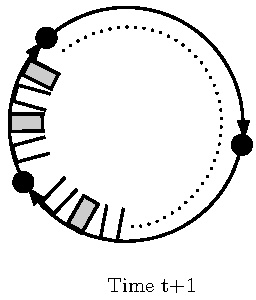
\includegraphics[scale=0.7]{containers2}
      \end{center}
delay

     \caption{Dynamic behavior of the ring.}\label{fig:containers}

  \end{figure}

     \paragraph{C-RAN traffic}

  We consider a set of $RRH$, each one connected to a node on the ring through an electronic interface of bit rate $R$ Bps (note that several RRHs can be attached to the same vertex). The RRHs are the source of the {\bf deterministic and periodic} C-RAN traffic.
Assume also that the bandwidth of the ring (i.e., the sum of capacities of all the containers) is at least equal to $F\times R$ Bps. The integer $F$ is called the {\bf acceleration factor} between the electronic and the optical domains. A node aggregates the data received on the electronic interface during $F$ units of time to create a  frame of data of size $C$ and then fills a container of the ring with this frame.

A period is fixed number of consecutive slots of time.  In each period $P$, an RRH emits data during a slot called \textbf{emission time} or $ET$. Hence the RRH emits $ET / F$ packets, i.e., a container of size $C$ each $F$ units of time during the emission time, see Figure \ref{fig:interface}. Consider that he data of the RRH $i$ arrives in a period at some node $u$ at a time $m_i$  called {\bf offset}. The offsets can be determined  by the designer of the system and can be different for each RRH but must remain the same over all periods. We assume that all BBUs are contained in the same data-center attached to a node $v$. The data from $u$ is routed to its BBU at node $v$ through the ring and arrives at time $m_i + \omega(u,v)$ if it has been inserted in the ring upon arrival. Then after some computation time (which w.l.o.g. is supposed to be zero), an answer is sent back from the BBU to the RRH. The same quantity of data (i.e. size of frame) is emitted by each BBU or RRH during any period.

   In this study the {\bf delay} of a message is defined as the time it waits in the origin node $u$   before being sent on the ring. The latency is thus the sum of the delay plus $\omega(u,v) $  where $v$ is the destination node.
   The aim of our study is to deterministically minimize the delay of the C-RAN traffic, both from the node connected to a target RRHs to the node connected to its  BBUs then from the BBU to the RRH (uplink and downlink traffic).
   In Section \ref{sec:deterministicalgorithms} we propose a deterministic mechanism with zero delay which preserves the latency of other data using the optical ring. We shortly describe the nature of this additional traffic in the next subsection.


\begin{figure}[h!]
\begin{center}

      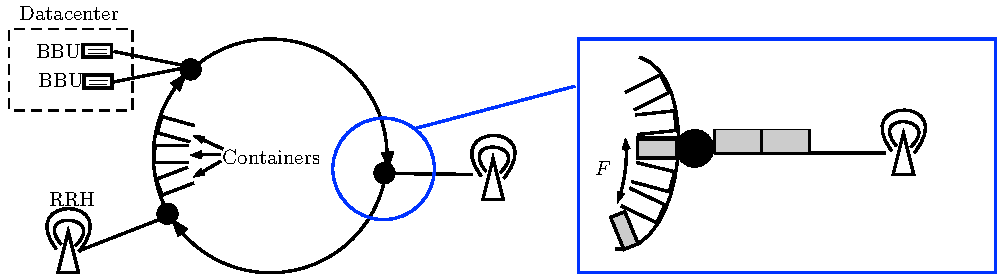
\includegraphics[scale=0.7]{interface.pdf}
     \caption{Insertion in the N-GREEN optical ring.}\label{fig:interface}

\end{center}
  \end{figure}


\paragraph{Best effort traffic}

The optical ring has to serve not only C-RAN traffic but also a Best effort traffic (BE).  This BE traffic has no latency constraints to be respected, but the  distribution of delays for this BE traffic is a measure of quality of the ring.  At each node of the ring, a insertion buffer is filled with BE packets to be sent on the ring by a batch arrival process generation. Indeed, as it is generated, each BE packet is inserted in a frame associated with its destination on the ring. When a frame is enough filled or enough old (depending on chosen fill rate and maximum waiting time parameters), it is ready to be inserted into an empty container on the ring.  The generation of BE packets is modeled by a temporal law that gives the distribution of times between two arrivals of a set  of BE packets in a node. The computation of this distribution for the parameters of the insertion buffer used in the N-GREEN optical ring is described in ~\cite{youssef2018}.

   \section{Evaluation of the delay on the N-GREEN optical ring}
   \label{sec:oportmethods}
   We considered different insertion policies of C-RAN and BE frames in empty containers on the ring.   BE frames obey an opportunistic insertion policy :  when BE frames are ready to be sent, the corresponding node insert them in a outgoing  empty container as soon as it can. If there are several  such waiting BE frames in  a node,  they are stored in an insertion buffer. Two different methods to manage this insertion buffer are experimentally compared. The FIFO rule is compared to a method that uses two insertion buffers : one for the BE frames, and another for the C-RAN frames. The C-RAN insertion buffer has priority  on the BE insertion buffer.  Figure \ref{fig:resultopport} gives the cumulative distribution of both C-RAN and BE traffics latencies for the FIFO rule and the "C-RAN first" rule. In this experiment, the offsets of the RRH are not fixed but randomly distributed in the period. The experimental parameters are given by Figure \ref{fig:params} and chosen following~\cite{ngreenarchitecture}. The results are computed over $100$ experiments (with different random offsets) where the optical ring is simulated during $10,000,000$ units of time. The source code in C of the experiments can be found in ~\cite{webpage}.

   \vspace{0.5cm}
  \hspace{-0.75cm}


        \begin{center}
      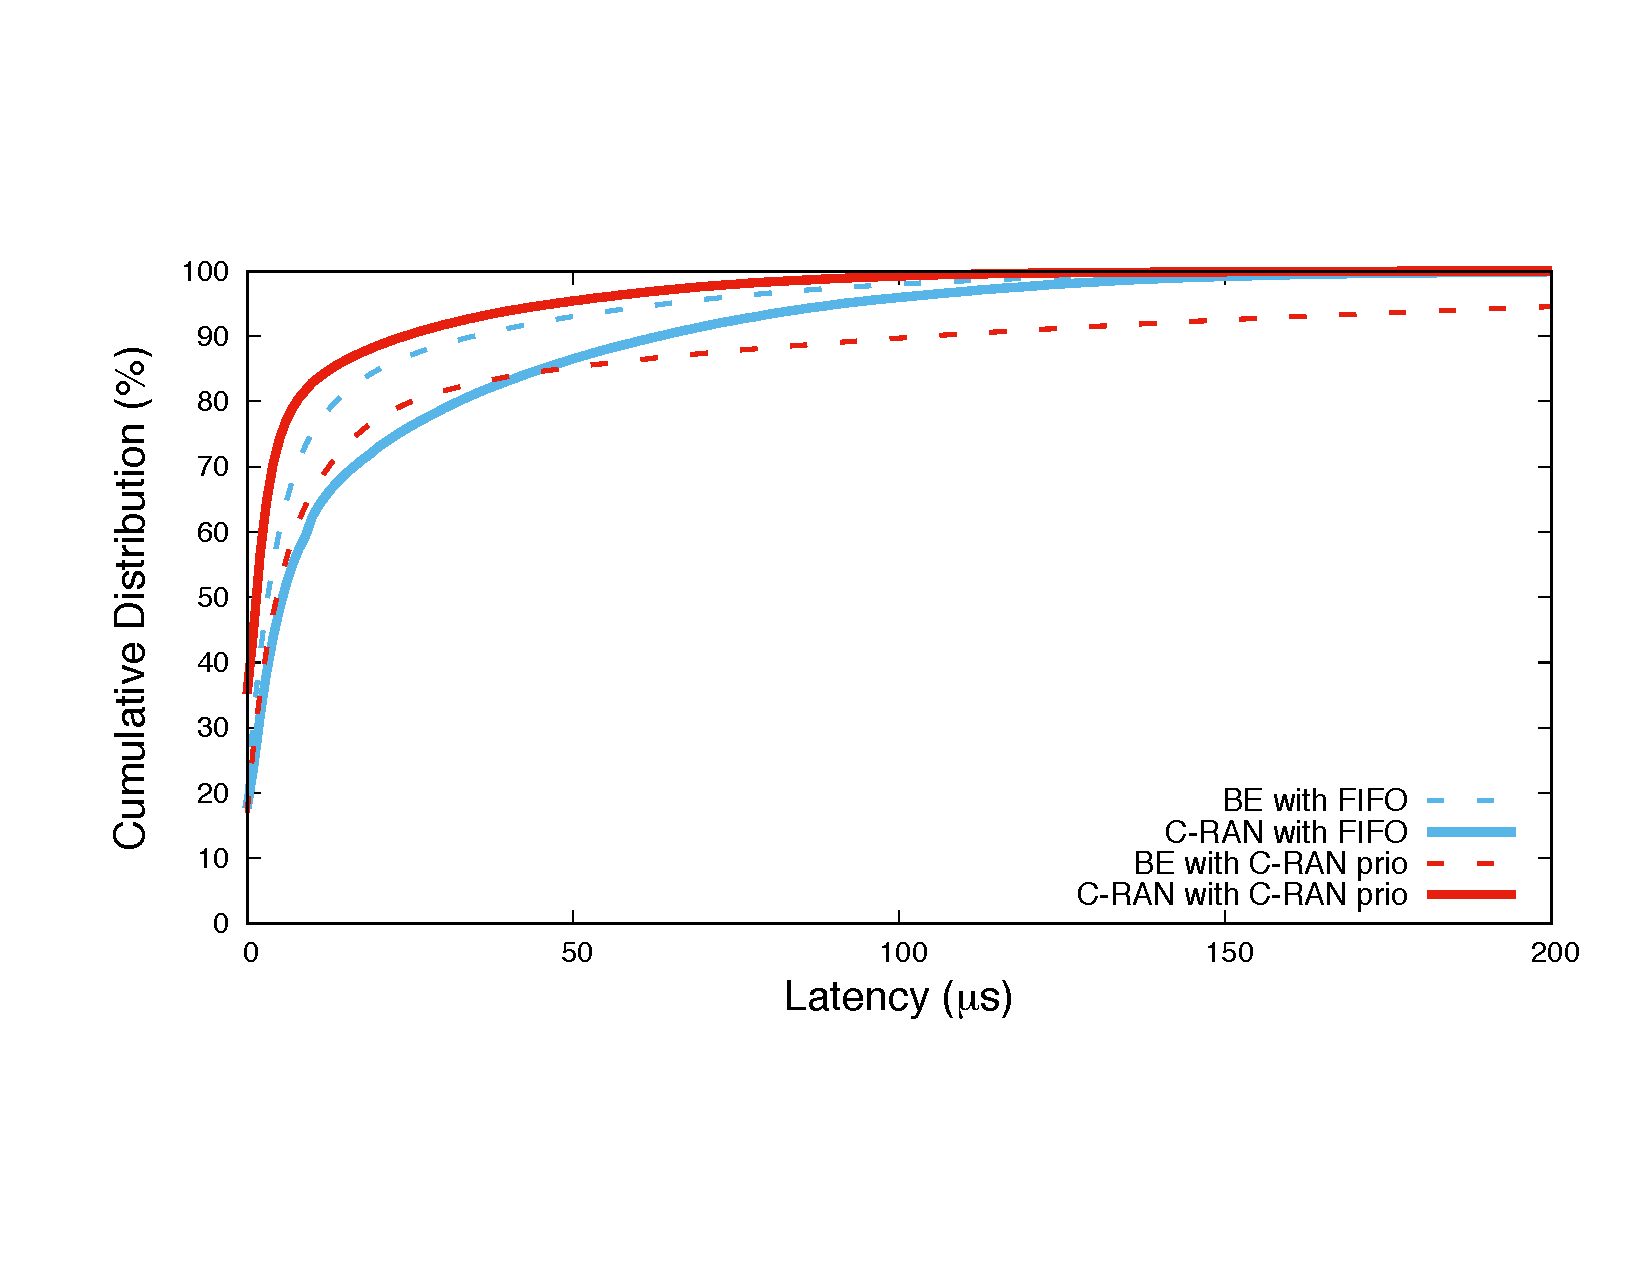
\includegraphics[scale=0.3]{opport.pdf}

     \captionof{figure}{Distribution of latencies for FIFO and C-RAN first}    \label{fig:resultopport}

  \scalebox{0.65}
  {

  \begin{tabular}{|c|c|}
  \hline
  Bit rate of an electronic interface $R$ & $10$ Gbps \tabularnewline
  \hline
  Optical ring bit rate $F\times R$ & $100$ Gbps \tabularnewline
  \hline
    Acceleration factor $F$ & $10$  \tabularnewline
  \hline
  Container size  $C$ & $100$ kb  \tabularnewline
  \hline
  Unit of time $C/(F\times R)$ & $1~\mu$s \tabularnewline
  \hline
  Length of the ring $RS$ & $100$ \tabularnewline
  \hline
  Emission time $ET$ & $500$ \tabularnewline
  \hline
   Period $P$ & $1,000$ \tabularnewline
  \hline
  Number of RRH & $5$  \tabularnewline
  \hline
  Number of nodes $n$ & $5$  \tabularnewline
  \hline
   Load induced by C-RAN traffic & $50\%$  \tabularnewline
  \hline
    Load induced by BE traffic & $40\%$  \tabularnewline
  \hline
  \end{tabular}
  }

  \captionof{figure}{Experimental parameters of the N-GREEN architecture}\label{fig:params}
      \end{center}

Unsurprisingly, the delay of the C-RAN traffic is better when we prioritize the C-RAN traffic, while the BE traffic is penalized. Nevertheless, there is still $10\%$ of the C-RAN traffic with a delay higher than $50 \mu$s, a problem we address in the next section.


\section{Deterministic approach for zero delay} \label{sec:deterministicalgorithms}

Finding good offsets for the C-RAN traffic is a hard problem even for simple topologies and without BE traffic, see~\cite{dominique2018deterministic}. In this section, we give a simple solution to this problem in the N-GREEN optical ring, and we adapt it to minimize the delay of the BE traffic.

Let $u$ be the node to which is attached the RRH $i$, to ensure zero delay for the C-RAN traffic, then the container which arrives at $u$ at time $m_i$ must be free so that the data from the RRH can be sent immediately on the optical ring.

To avoid delay between the arrival of the data from the RRH and its insertion on the optical ring,
we allow nodes to \textbf{reserve} a container one round before using it. A container which is reserved cannot be filled by any node except the one which has reserved it (but it may contain data when it is reserved).
Let $u$ be the node to which is attached the RRH $i$, if $u$ reserves the container $u$ at time $m_i - RS$, then it is guaranteed that $u$ can fill a free container at time $m_i$ with the data of the RRH $i$.
In the method we now describe, the C-RAN packets never wait in the node: the message sent by the RRH $i$ arrives at its BBU at node $v$ at time $m_i + \omega(u,v)$ and the answer is sent from the BBU at time $m_i + \omega(u,v) +1$.

Recall that an RRH fills a container every $F$ units of time, during a time $ET$.
Thus if we divide the period $P$ into \textbf{slots} of $F$ consecutive units of time, an RRH needs to use at most one container by slot. If an RRH emits at time $m_i$, then we say it is at \textbf{position} $m_i + \omega(u,v)\pmod F$.
The position of an RRH corresponds to the position in a slot of the container it has emitted, when it arrives at $u$.
If an RRH is at position $p$, then by construction, the corresponding $BBU$ is at position $p+1\pmod F$. Since we do not allow waiting times for C-RAN traffic, each RRH uses a container at the same position during all the period.

The problem we solve now is to find an \textbf{assignment} of values of the $m_i$'s which is \textbf{valid}: two RRHs never reserve or use the same container in a period. Moreover we want to preserve the delay of the BE traffic. It means that the time a node waits for a free container at any point of the period must be minimized.
Remark that two RRHs which are not connected to a same node on the ring never use the same containers. Moreover, if we fix the offsets of the RRHs to even positions so that they do not reserve the same containers, then it will fix the offsets of the BBUs to odd positions which do not reserve the same containers. Hence we need to deal with the RRHs only.


\begin{prop}
\label{prop:assign}
There is an assignment of the offsets $m_1, \dots, m_k$ on the same position if  $k\times ET + RS \leq P$.
\end{prop}
\begin{proof}
 W.l.o.g we fix $m_1$ so that it is at position $0$ and all the other offsets will then be chosen at position $0$.
 Let $u_1,\dots,u_k$ be the nodes attached to the RRHs $1,\dots,k$. We assume that $u_1,\dots,u_k$ are in the order of the ring. The last message emitted by the RRH $1$ arrives at $u_2$ at time $ET - 1 + \omega(u_1,u_2)$. Therefore we can fix $m_2 = ET  + \omega(u_1,u_2)$. In general we can set $m_i = (i-1) \times ET + \omega(u_1,u_i)$ and all RRHs will use different containers at position $0$ during a period. Since $k \times ET + \omega(u_1,u_1) \leq P$ by hypothesis,
 the containers filled by the $k$th RRH are freed before $P$. Hence when the RRH $1$ must emit something in the second period, there is a free container.\qed
\end{proof}

From this proposition, it is easy to derive the maximal number of antennas which can be supported by an optical ring,
when using reservation and the same position for an RRH for the whole period.

\begin{corollary}
The maximal number of RRH such that there is an assignment is $ \lfloor\frac{P- RS}{ET}\rfloor \times \frac{F}{2}$.
\end{corollary}
\begin{proof}
Following Prop.~\ref{prop:assign}, the number of antennas on a position is $k = \lfloor\frac{P- RS}{ET}\rfloor $.
Since we need two positions for $k$ antennas, in order to carry the traffic coming from the RRHs and the BBUs, and we got $F$ positions in the slot, the number of antennas supported by the ring is thus equal to $k \times \frac{F}{2}$.\qed
\end{proof}


We now present an algorithm using reservation as in Proposition \ref{prop:assign} to set the offsets at the same position.
In the naive version of the algorithm, we put each RRH in an arbitrary position, for instance one RRH by position.
 We then propose three ideas to optimize the latency of the BE traffic, by spacing as well as possible the free containers in a period.


\paragraph{Packing}

For each position which is used by some RRH, and during each period, $RS$ containers are reserved before starting to emit some C-RAN traffic, while they are free. Hence, it decreases the maximal load the system can handle.
Therefore to not waste bandwidth, it is relevant to put as many RRHs as possible on the same position as in Figure \ref{fig:packing}. Indeed, for any position which is not used at all, $RS$ containers need not to be reserved. This strategy is also good for the latency of the BE traffic. If a position is unused, then there is always a container free of C-RAN traffic each $F$ unit of times.

\begin{figure}[h!]
\begin{center}

      \includegraphics[scale=0.5]{repart0}
     \caption{Packing.}\label{fig:packing}

\end{center}
  \end{figure}

\paragraph{Balancing inside the slot}

The free positions can be distributed uniformly over a slot, to minimize the time to wait before a node
has access to a free container, as shown in Figure~\ref{fig:slotbal}. It is a small optimization, since
it decreases the delay of at most $F/2$.

\begin{figure}[h!]
\begin{center}

      \includegraphics[scale=0.55]{repart1}
     \caption{Balancing inside the slot.}\label{fig:slotbal}

\end{center}
  \end{figure}
\paragraph{Balancing inside the period}

It is possible that there are no unused position as it happens with the parameters of the N-GREEN ring given in Figure~\ref{fig:params}: $ET = \frac{P}{2}$, $F = 10$ and $n = 5$. Any assignment has exactly one  BBU or RRH at each position. If all the RRHs start to emit in the first slot, then during $ET$ there will be no free containers anywhere on the ring, inducing a huge delay for the BE traffic.
To mitigate this problem, in a period, the time with free containers in each position must be uniformly distributed over the period as shown in  Figure~\ref{fig:periodbal}.
\begin{figure}[h!]
\begin{center}

      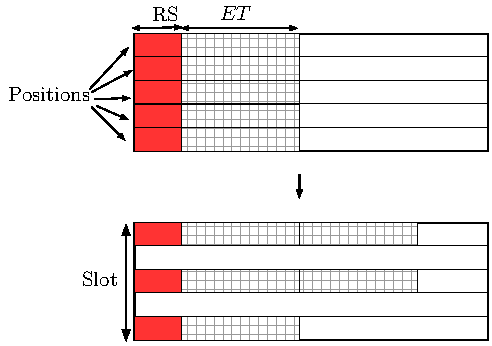
\includegraphics[scale=0.55]{repart2}
     \caption{Balancing inside the period.}\label{fig:periodbal}

\end{center}
  \end{figure}
  \paragraph{Experimental evaluation}

To evaluate the effectiveness of the allocation approach proposed here, we will compare its performances in terms of delays with the ones of several methods without allocation. So in order to understand the contribution of the three approaches presented in the previous subsection, we first give the cumulative distribution of the delay of the BE traffic  in Figure \ref{fig:algocmp}. To evaluate the performances of  the  N-GREEN ring when   several RRHs are connected to a same node on the ring, the parameter $ET$ has been set to $400$.

The performance with the no packing approach is really bad, even worst than the methods using an insertion buffer. It is explained by the parameters of the N-GREEN ring: all positions are used and thus, there are no free containers available to BE traffic during $ET+RS$ units of time. When packing the RRHs on a minimal number of positions, the delay decreases dramatically and becomes much better than in the previous methods. The optimizations of spacing inside the slot brings almost no benefit as expected. The spacing over a period improves the delay marginally. In settings with an higher load, spacing inside a period would have a much larger effect.

In Figure \ref{fig:optimres}, we compare the cumulative distribution of the delay of the BE traffic using the FIFO rule or the reservation algorithm proposed here. To keep the load at $90\%$ as in the experiment of  Figure~\ref{fig:resultopport}, we set $ET = 200$ and $n = 12$. This is not out of context since the exact split of the C-RAN (the degree of centralization of the computation units in the cloud) is not fully determined yet~\cite{mobile2011c}. With these parameters, the loss of bandwidth due to reservation is at most $6\%$

\begin{center}
      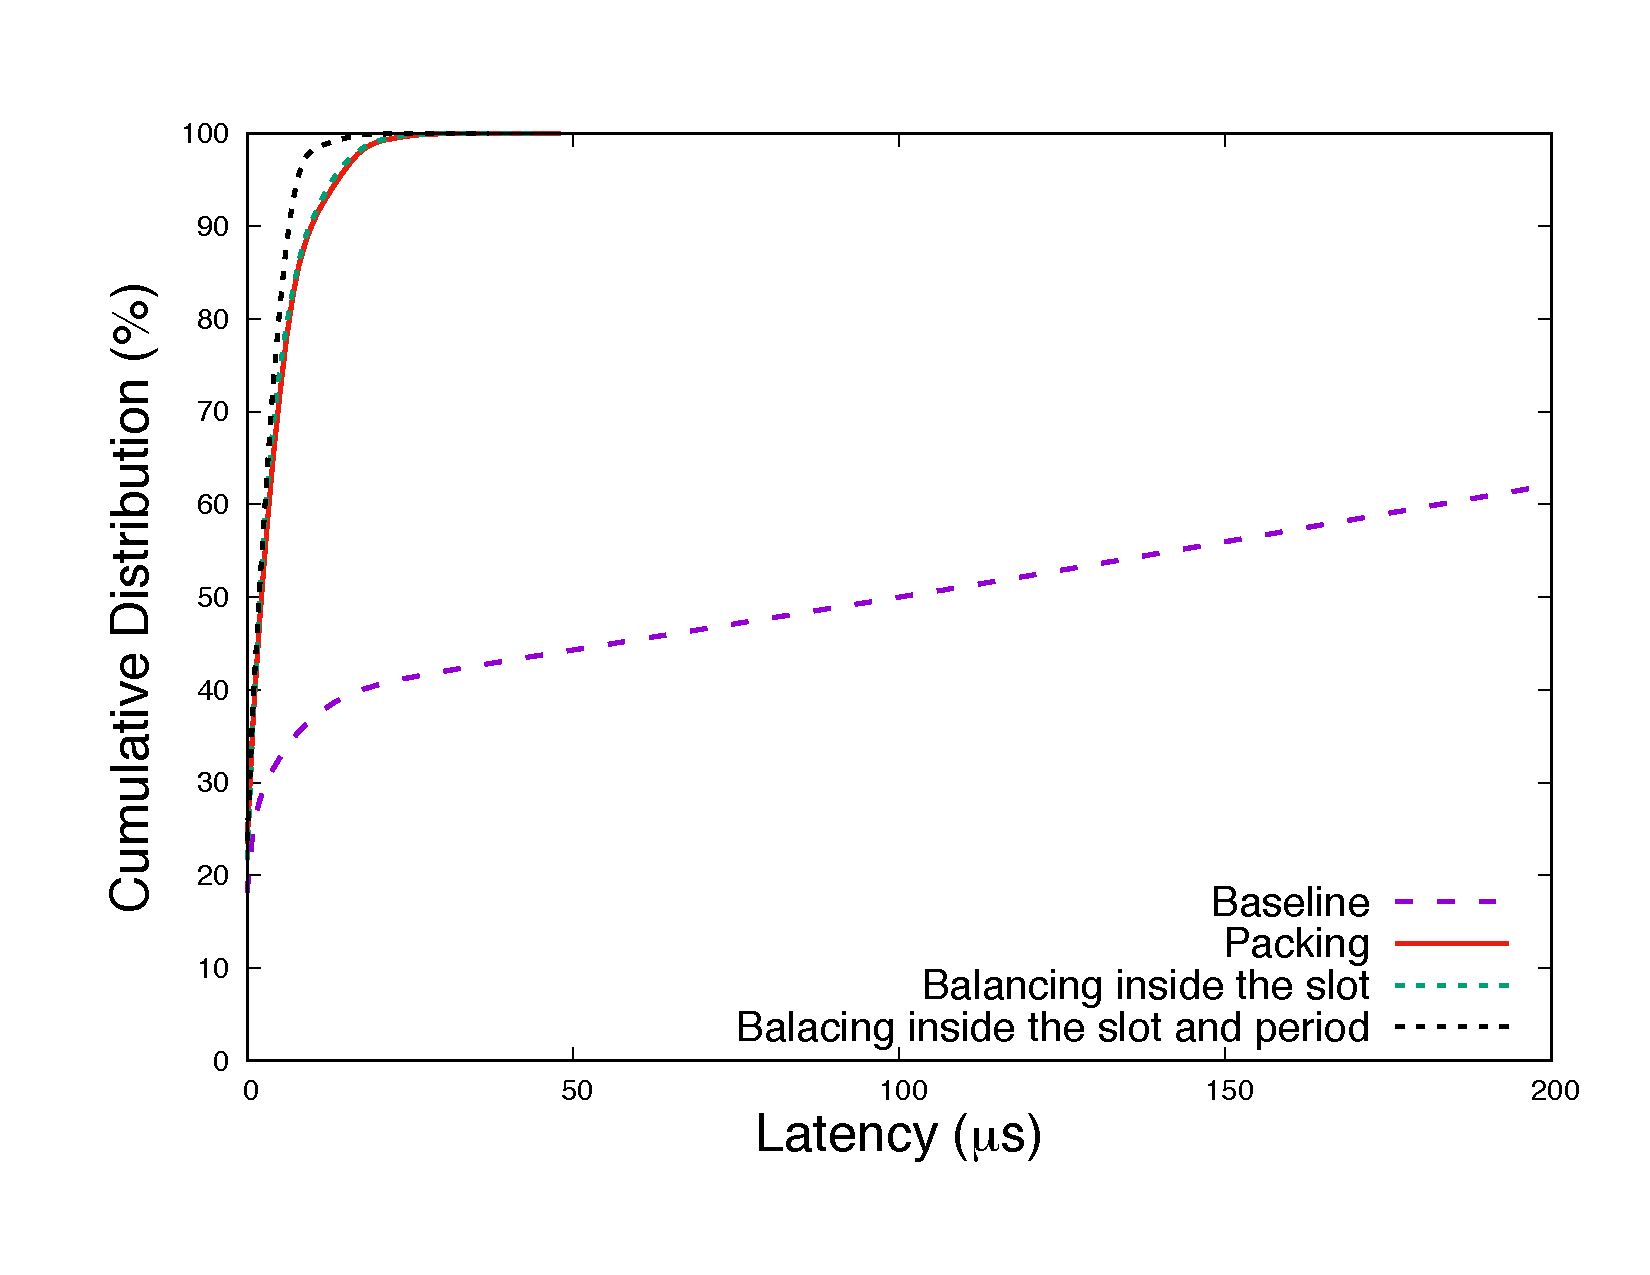
\includegraphics[scale=0.25]{repart1res}
     \captionof{figure}{Impact of the repartition on the delay.} \label{fig:algocmp}

\vspace{0.5cm}

      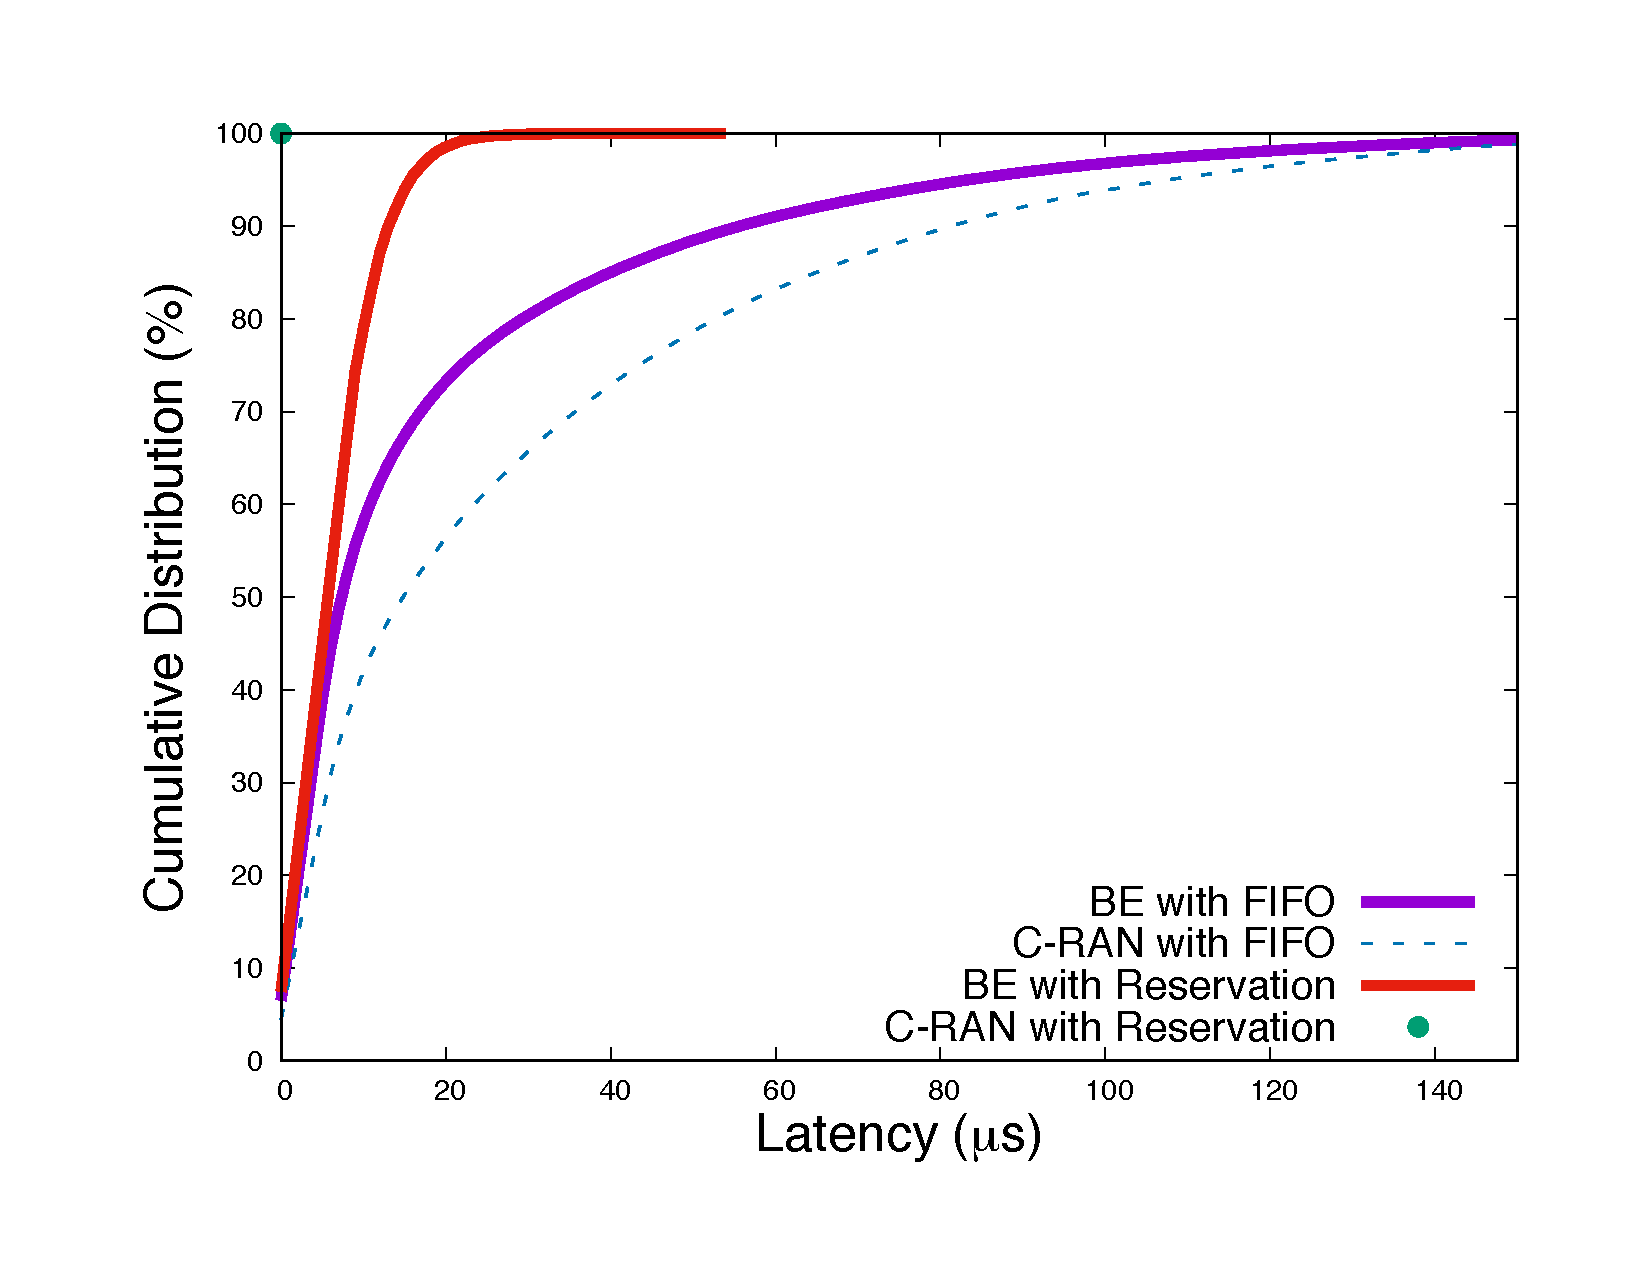
\includegraphics[scale=0.25]{optim.pdf}
     \captionof{figure}{Impact of the deterministic method on the traffics.}   \label{fig:optimres}

\end{center}
  The performance of the reservation algorithm is excellent, since the C-RAN traffic has {\bf zero delay} and the BE traffic has a \textbf{better delay} with reservation than with the FIFO rule. It is due to the balancing of the load of the C-RAN traffic over the period, that guarantee a more regular bandwidth for the BE traffic.



  \bibliographystyle{ieeetr}
\bibliography{src}

\end{document}
\bibitem{Sz16} T. H. Szymanski. An Ultra-Low-Latency Guaranteed-Rate Internet for Cloud Services. IEEE/ACM TRANSACTIONS ON NETWORKING, VOL. 24, NO. 1, FEBRUARY 2016

